\title{
	02239 Data Security\\
	----- Access Control Lab -----
	}
\author{
Casper Sloth Paulsen (s110448)\hspace{1cm}
\includegraphics[scale=.2]{csp.png}\\
Stefan Mertens (s113420)\hspace{1cm}
\includegraphics[scale=.1]{stm.png}\\
Anders Rydbirk (s113725)\hspace{1cm}
\includegraphics[scale=.35]{img/anders_signature.png}
}
\date{\today}

\documentclass[12pt]{article}
\usepackage[T1]{fontenc} % the font encoding
\usepackage[utf8]{inputenc} % the input encoding
\usepackage{lmodern} % the Latin Modern font
\usepackage{graphicx}
\usepackage{geometry}
\usepackage{listings}
\usepackage{color}
\usepackage{xcolor}

\definecolor{bluekeywords}{rgb}{0.13,0.13,1}
\definecolor{greencomments}{rgb}{0,0.5,0}
\definecolor{turqusnumbers}{rgb}{0.17,0.57,0.69}
\definecolor{redstrings}{rgb}{0.5,0,0}
\definecolor{dkgreen}{rgb}{0.0,0.35,0}
\definecolor{dred}{rgb}{0.545,0,0}
\definecolor{dblue}{rgb}{0,0,0.545}
\definecolor{lgrey}{rgb}{0.9,0.9,0.9}
\definecolor{gray}{rgb}{0.4,0.4,0.4}
\definecolor{darkblue}{rgb}{0.0,0.0,0.6}

\lstdefinelanguage{FSharp}{
      backgroundcolor=\color{black!5},  
      basicstyle=\small \ttfamily \color{black} \bfseries,   
      breakatwhitespace=false,       
      breaklines=true,               
      captionpos=b,                   
      commentstyle=\color{dkgreen},   
      deletekeywords={...}, 
      escapeinside={\%*}{*)},                  
      frame=single,                  
      language=TeX, 
      morekeywords={let, new, match, with, rec, open, module, namespace, type, of, member, 			and, for, in, do, begin, end, fun, function, try, mutable, if, then, else},
    keywordstyle=\color{bluekeywords},
    sensitive=false,
    morecomment=[l][\color{greencomments}]{///},
    morecomment=[l][\color{greencomments}]{//},
    morecomment=[s][\color{greencomments}]{{(*}{*)}},
    morestring=[b]",
    stringstyle=\color{redstrings},			%Insert missing keywords here
      emphstyle=\color{cyan},               
      keywordstyle=\color{blue}, 
      identifierstyle=\color{redstrings},
      stringstyle=\color{blue},      
      numbers=none,                 
      numbersep=5pt,                   
      rulecolor=\color{black},        
      showspaces=false,               
      showstringspaces=false,        
      showtabs=false,                
      stepnumber=1,                   
      tabsize=4,
      columns=fullflexible,                
      title=\lstname
}
\geometry{
 a4paper,
 total={210mm,297mm},
 left=25mm,
 right=25mm,
 top=5mm,
 bottom=20mm,
 }

\begin{document}
\clearpage\maketitle
\thispagestyle{empty}

%\begin{center}
%----- End of assignment -----
%\end{center}
\section*{Brief reflection}
The goal of this project was to make a game called Nim, in which a player plays against the computer. To achieve this we used the reactive programming paradigm. Beyond making the basic game, we added a dynamic AI, communication with an external web service, and an easy to use GUI. 

The game consists of the three parts, GUI, Dialogue, and Game, which each have separate concerns. GUI handles the user interface, Dialogue handles user input, and Game handles game operations. Because they each have separate concerns, each part is loosely coupled to the others. This was in part achieved by using the reactive programming paradigm and signature files to hide the implementation details from other parts of the program. Because of this, both the Game and Dialogue doesn't know about the GUI which means that a new GUI could be developed without it affecting the Dialogue or Game logic. The GUI communicates with the Dialogue through an ingoing event queue and receives updates in an outgoing event queue. This is the part that makes it possible to separate the GUI from the rest of the program, as the two event queues serve as a communication line. Both the Dialogue and GUI are asynchronous. 

Since the game is asynchronous, all types in the Game part are immutable, as this avoids a lot of problems in asynchronous programming. 

Originally the AI would always make the most optimal move, but this was a bit boring, and in order to make the game more fun we decided to make an AI that has a dynamic difficulty. What this means is that the AI actually makes small mistakes which makes the game a bit more fun to play.
\begin{figure}[h]
\begin{center}
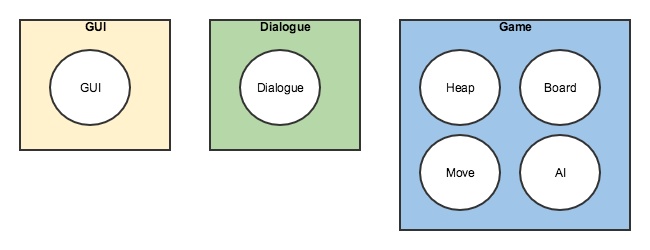
\includegraphics[scale=.45]{img/modules.png}
\caption{The main modules}
\end{center}
\label{fig:modules}
\end{figure}
We also made an external web service, implemented in a functional language, which returns a random new game. This could be extended for a future online multiplayer game.

In general we tried to make the GUI as easy to use as possible. We think we have a achieved this. An improvement would be to show possible error messages. However the game is designed in a way to avoid errors in general.
    

\section*{Main types}

\lstset{language=FSharp}
\begin{lstlisting}
//module Nim.Game.Heap
type heap = H of int
//module Nim.Game.Board
type board = B of heap list
//see other types in the signatures section
    \end{lstlisting}

\section*{AI}
The AI gives the human player a fair chance, by having a probability to make a mistake (random valid move) which decreases over time. See figure 2.


\section*{Signatures for the main functions}
\begin{lstlisting}
module Nim.Game.Board
type board
val move : index:int -> count:int -> board:board -> Choice<string,board>
val iter: (heap -> unit) -> board -> unit
val make : int -> int -> board
val item : int -> board -> heap
val isGameOver : board -> bool
val numberOfHeaps: board -> int
val numberOfMatches: board -> int
val makeWeb: string -> board
val fold: ('a -> heap -> 'a) -> i:'a -> board -> 'a
val map: (heap -> 'a) -> board -> 'a 
\end{lstlisting}
\begin{figure}[!h]
\begin{center}
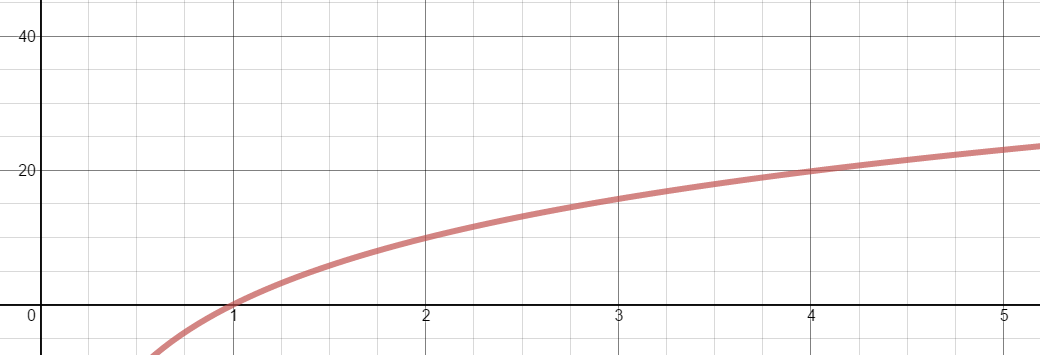
\includegraphics[scale=.40]{graphlogx.png}
\caption{The AI difficulty function: $P(mistake) = 33\% \times log^{10}(\frac{\sum matches} {\sum heaps} )$}
\end{center}
\label{fig:ai}
\end{figure}
\begin{lstlisting}
module Nim.Dialogue
type InputMessage =
    | NewGame of int * int | Move of int * int | Download | DownloadComplete of string | Cancel | Cancelled | DownloadError  | Done of Choice<string,board> | Forfeit
type OutputMessage =
    | CreateGame of board | Update of board | GameOver of string | Error of string | Downloading
val evIn : AsyncEventQueue<InputMessage>
val evOut : AsyncEventQueue<OutputMessage>
\end{lstlisting}
\begin{figure}[ht]
\begin{center}
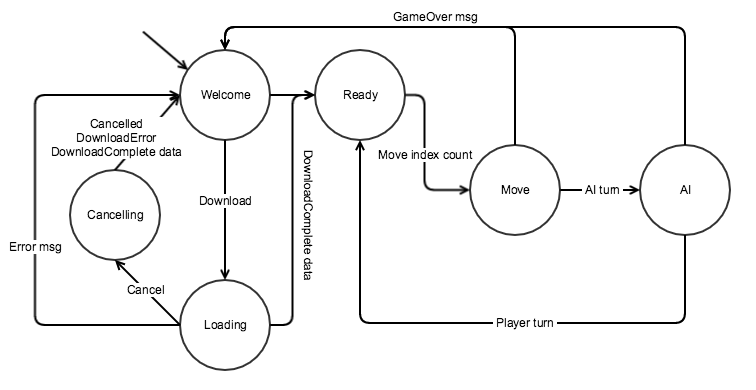
\includegraphics[scale=.64]{img/state_machine_nim.png}
\caption{The dialogue module automaton}
\end{center}
\label{fig:automaton}
\end{figure}

\begin{figure}[ht]
\begin{center}
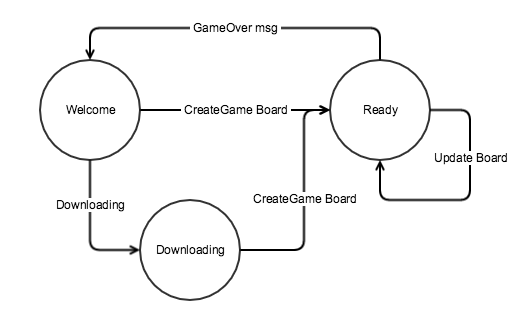
\includegraphics[scale=.65]{img/gui_state_machine_nim.png}
\caption{The GUI automaton}
\end{center}
\label{fig:automaton}
\end{figure}


\end{document}